\section{常见函数的导数-上}\label{013}

\begin{tcolorbox}[size=fbox, breakable, enhanced jigsaw, title={指数函数}]

从指数函数开始, 首先考虑自然常数作为底数的情况, 代入导数的定义:
\begin{align*}
\frac{\mathrm{d}}{\mathrm{d}x}(\mathrm{e}^x)=&\lim_{h\rightarrow0}\frac{\mathrm{e}^{x+h}-\mathrm{e}^x}{h}\\
=&\lim_{h\rightarrow0}\mathrm{e}^x\left(\frac{\mathrm{e}^h-1}{h}\right)\\
&\text{令 }n:=1/h\\
=&\lim_{n\rightarrow\infty}\mathrm{e}^x\left(\frac{\mathrm{e}^{1/n}-1}{1/n}\right)\\
&\text{根据定义 }\mathrm{e}\equiv\lim_{n\rightarrow\infty}\left(1+\frac{1}{n}\right)^n\\
=&\lim_{n\rightarrow\infty}\mathrm{e}^x\left(\frac{{\left(\left(1+1/n\right)^n\right)}^{1/n}-1}{1/n}\right)\\
=&\lim_{n\rightarrow\infty}\mathrm{e}^x\left(\frac{1+1/n-1}{1/n}\right)\\
=&\mathrm{e}^x.
\end{align*}
于是
\begin{equation*}
    \boxed{\frac{\mathrm{d}}{\mathrm{d}x}\mathrm{e}^x=\mathrm{e}^x}.
\end{equation*}

对于其他的底数, 例如 $a^x$, 我们需要一些额外的知识了:

\begin{tcolorbox}[size=fbox, breakable, enhanced jigsaw, title={链式法则 chain rule}]

结论上有: 
\begin{equation*}
    \boxed{\frac{\mathrm{d}y}{\mathrm{d}x}=\frac{\mathrm{d}y}{\mathrm{d}u}\frac{\mathrm{d}u}{\mathrm{d}x}}.
\end{equation*}

\end{tcolorbox}

\begin{newquote}
即原先有一个函数 $y=h(x)$, 将它改写为一个符合函数 $y=f(g(x))$, 并令
$u:=g(x)$.

不严格的直觉上的证明:

$\Delta u=g(x+\Delta x)-g(x)$, $\Delta y=f(u+\Delta u)-f(u)$. 于是
$\frac{\Delta y}{\Delta x}=\frac{\Delta y}{\Delta u}\frac{\Delta u}{\Delta x}$.
再取 $\Delta x\rightarrow0$ 的极限, 若 $g(x)$ 是连续的, 在
$\Delta x\rightarrow0$ 时便有 $\Delta u\rightarrow 0$,
于是便得到了上述结论.
\end{newquote}

现在我们再来看 $a^x$, 我们可以先利用\ref{002}\nameref{002}的知识换个底数,
$a^x=\mathrm{e}^{\ln(a)x}$, 再利用链式法则, 令 $y:=\mathrm{e}^u$
$u:=\ln{(a)}x$, 于是
\begin{align*}
\frac{\mathrm{d}}{\mathrm{d}x}(a^x)=&\frac{\mathrm{d}y}{\mathrm{d}u}\frac{\mathrm{d}u}{\mathrm{d}x}\\
=&(\mathrm{e}^u)(\ln{a})\\
=&(\ln{a})\mathrm{e}^{\ln{a}}=(\ln{a})a^x.
\end{align*}

更加通常 (generalize) 一点, 我们可以有
\begin{equation*}
\boxed{\frac{\mathrm{d}}{\mathrm{d}x}a^{u(x)}=(\ln{a})a^u\frac{\mathrm{d}u}{\mathrm{d}x}}.
\end{equation*}

\end{tcolorbox}

\begin{tcolorbox}[size=fbox, breakable, enhanced jigsaw, title={三角函数}]

先考虑 $\sin$,
\begin{align*}
\frac{\mathrm{d}}{\mathrm{d}x}(\sin(x))=&\lim_{h\rightarrow0}\frac{\sin(x+h)-\sin(x)}{h}\\
\text{ 参见\ref{010}\nameref{010}, }\sin(a\pm b)=\sin a\cos b\pm \cos a\sin b\\
=&\lim_{h\rightarrow0}\frac{\sin(x)\cos(h)+\cos(x)\sin(h)-\sin(x)}{h}\\
=&\lim_{h\rightarrow0}\left(\frac{\sin(x)(\cos(h)-1)}{h}+\frac{\cos(x)\sin(h)}{h}\right),
\end{align*}

到这一步似乎就不很直观了, 若是直接取 $h=0$, 则有 $\cos(h)-1=0$ 和
$\sin(h)=0$, 两项的分子分母都同时为零了, 类似这种出现了
$\frac{0}{0}$ 或者 $\frac{\infty}{\infty}$ 的情况称为不定式/未定型
(indeterminate forms), 后面我们会看到将有一种更便 (简单) 捷 (粗暴)
的方式来解决这样的问题 (剧透: 洛必达法则 - L\'H\^{o}pital's rule),
目前我们先老老实实地来解决. 对于上面的形式, 我们可以用几何方法入手:

\begin{tcolorbox}[size=fbox, breakable, enhanced jigsaw, sidebyside]
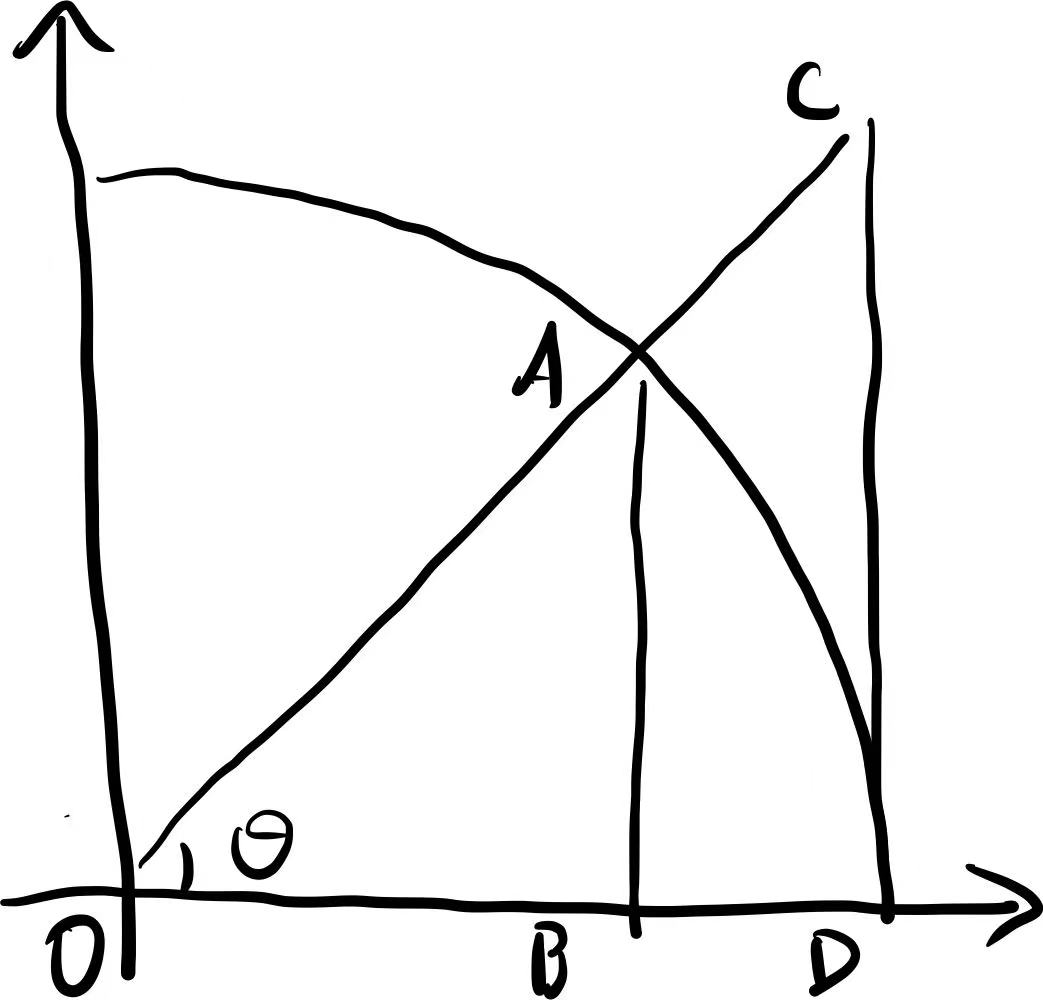
\includegraphics[width=0.9\textwidth]{img/image-20230529100555673.png}
\tcblower
\kaishu{\small 如左图所示, 考虑一个单位圆, 三角形 $OAB$, 扇形 $OAD$, 和三角形
$OCD$ 的面积关系是 $\sin(\theta)/2<\theta/2<\tan(\theta)/2$;
将每个式子都除以 $\sin(\theta)/2$, 有
$1<\theta/\sin(\theta)<1/\cos(\theta)$; 再取倒数, 得到
$1>\sin(\theta)/\theta>\cos\theta$.
这个结论至少在第一象限应该是成立的, 于是当我们取 $\theta=0$ 时,
我们发现不等式的最右边也是 $1$ 了, 直觉上, 中间一项既要比 $1$ 小,
又要比 $1$ 大, 那么它只能是等于 $1$ 了. 这个朴素的想法被叫做
``三明治定理'' (Sandwich Theorem, 也叫夹逼定理\ldots).}
\end{tcolorbox}

这样一来, 便有当 $h\rightarrow0$, $\sin(h)/h\rightarrow 1$,
另一项的话, 也不难利用三角函数的恒等式变形:
\begin{align*}
&\frac{\cos(h)-1}{h}\\
&\text{参见\ref{010}\nameref{010}}\cos2a=1-2\sin^2a\\
=&-\frac{2\sin^2(h/2)}{h}\\
&\text{令 }\theta:=h/2\\
=&-\frac{\sin(\theta)}{\theta}\cdot\sin(\theta),
\end{align*}

于是当 $h\rightarrow0$, $\theta\rightarrow0$,
\begin{align*}
&\frac{\cos(h)-1}{h}\\
=&-\frac{\sin(\theta)}{\theta}\cdot\sin(\theta)\\
=&-(1)\cdot(0)\\=&0.
\end{align*}
综上,
\begin{equation*}
    \boxed{\frac{\mathrm{d}}{\mathrm{d}x}(\sin(x))=\cos(x)}.
\end{equation*}

类似的, 不难推出
\begin{equation*}
    \boxed{\frac{\mathrm{d}}{\mathrm{d}x}(\cos(x))=-\sin(x)}.
\end{equation*}

利用上面两个结论和除法法则等, 也不难继续得到下面的结论, 过程留作练习.
$$\boxed{\begin{aligned}&\frac{\mathrm{d}}{\mathrm{d}x}\tan(x)=\sec^2(x),\\
&\frac{\mathrm{d}}{\mathrm{d}x}\cot(x)=-\mathrm{cosec}^2(x),\\
&\frac{\mathrm{d}}{\mathrm{d}x}\sec(x)=\sec(x)\tan(x),\\
&\frac{\mathrm{d}}{\mathrm{d}x}\mathrm{cosec}(x)=-\mathrm{cosec}(x)\cot(x).\end{aligned}}$$

\end{tcolorbox}